\chapter{Структура Экосистемы OSTIS}
\chapauthortoc{Загорский А.~Г.\\Голенков В.~В.\\Шункевич Д.~В.}
{\label{chapter_ecosystem}}

\vspace{-7\baselineskip}

\begin{SCn}
\begin{scnrelfromlist}{автор}
	\scnitem{Загорский А.~С.}
	\scnitem{Голенков В.~В.}
	\scnitem{Шункевич Д.~В.}
\end{scnrelfromlist}

\bigskip

\scntext{аннотация}{Рассмотрена структура \textit{цифровой экосистемы} \textit{интеллектуальных компьютерных систем} на основе \textit{Технологии OSTIS}. Уточнена формальная трактовка таких понятий как \textit{ostis-система}, \textit{ostis-сообщество}, выделена типология \textit{ostis-систем}, что в совокупности позволяет определить структуру \textit{Экосистемы OSTIS}.}

\bigskip

\begin{scnrelfromlist}{подраздел}
	\scnitem{\ref{sec_ecosystem_structure}~\nameref{sec_ecosystem_structure}}
	\scnitem{\ref{sec_ostis_scientific_portal}~\nameref{sec_ostis_scientific_portal}}
	\scnitem{\ref{sec_corporate_ostis_system}~\nameref{sec_corporate_ostis_system}}
	\scnitem{\ref{sec_ostis_assistant}~\nameref{sec_ostis_assistant}}
\end{scnrelfromlist}


\bigskip
\begin{scnrelfromlist}{ключевой знак}
	\scnitem{Экосистема OSTIS}
\end{scnrelfromlist}

\begin{scnrelfromlist}{ключевое понятие}
	\scnitem{распределенная система}
	\scnitem{цифровая экосистема}
\end{scnrelfromlist}


\bigskip
\begin{scnrelfromlist}{библиографическая ссылка}
	\scnitem{\scncite{Briscoe2008}}
	\scnitem{\scncite{Boley2007}}
	\scnitem{\scncite{Masahary2018}}
	\scnitem{\scncite{Mohseni2021}}
	\scnitem{\scncite{Berners2001}}
	\scnitem{\scncite{Kiranne2018}}
	\scnitem{\scncite{Mccooi2006}}
	\scnitem{\scncite{Nacer2014}}
	\scnitem{\scncite{Burstrom2022}}
\end{scnrelfromlist}
\end{SCn}


\section*{Введение в Главу \ref{chapter_ecosystem}}

Понятие \textit{цифровой экосистемы} представляет собой сложную и динамичную систему, которая состоит из множества компонентов, включая технологии, процессы, пользователей, предприятия и многое другое. В контексте цифровых технологий переход к \textit{цифровой экосистеме} является ключевым аспектом для достижения целей бизнеса и общества.

Понятие \textit{цифровой экосистемы} можно определить как совокупность цифровых продуктов и сервисов, которые взаимодействуют друг с другом и с внешней средой, образуя единую среду обитания. Реализация \textit{цифровой экосистемы} сильно связано с формированием \textit{распределенной системы}. Такой принцип реализации имеет как преимущества (высокий уровень адаптивности, устойчивости, связности), так и недостатки (неоптимальность, неуправляемость, непредсказуемость поведения) (см. \scncite{Briscoe2008}, \scncite{Boley2007}, \scncite{Burstrom2022}). В отличие от полностью иерархически контролируемых систем, \textit{цифровая экосистема} представляет собой децентрализованную структуру, которая обеспечивает более гибкое и устойчивое управление (см. \scncite{Masahary2018}).

При традиционных подходах к решению проблемы формирования \textit{цифровой экосистемы} возникают проблемы, связанные с низким уровнем \textit{интероперабельности} таких систем (см. \scncite{Li2012a}). Традиционные подходы к решению данной проблемы зачастую неэффективны, поскольку каждая из систем имеет свой специализированный программный интерфейс и формат данных для взаимодействия. Это приводит к дополнительным расходам на устранение недостатков таких проблем. Поддержка жизненного цикла и модификация уже существующих систем может также потребовать дополнительных временных и ресурсных затрат.

Использование современных подходов к формированию \textit{цифровой экосистемы}, таких как открытые стандарты и протоколы взаимодействия, может значительно упростить задачу обеспечения \textit{интероперабельности} между различными системами. Это позволяет повысить эффективность и экономическую целесообразность проектов цифровой трансформации, снизить временные и финансовые затраты на разработку и поддержку \textit{цифровой экосистемы} (см. \scncite{Mohseni2021}). Однако стоит отметить, что даже при принятии идей семантического веба (см. \scncite{Berners2001}) могут возникнуть некоторые проблемы или ограничения, которые необходимо учитывать (см. \scncite{Kiranne2018}, \scncite{Mccooi2006}, \scncite{Nacer2014}).

\textit{Технология OSTIS} предоставляет возможности для создания \textit{цифровых экосистем}. Она обеспечивает эффективное управление данными и знаниями, обеспечивает автоматическую обработку информации и позволяет создавать интеллектуальные системы, способные обмениваться данными и знаниями между собой.

В данной главе монографии рассмотрена архитектура \textit{Экосистемы OSTIS} и её основных компонентов, методы разработки коллективов \textit{ostis-систем}, а также типология \textit{ostis-систем}, входящих в состав \textit{Экосистемы OSTIS}. Основная цель - предоставить полное представление о возможностях создания \textit{цифровых экосистем} на примере \textit{Экосистемы OSTIS}.

\section{Иерархическая система взаимодействующих ostis-сообществ}
{\label{sec_ecosystem_structure}} 

\begin{SCn}


\begin{scnrelfromlist}{ключевое понятие}
    \scnitem{ostis-система}
    \scnitem{самостоятельная ostis-система}
    \scnitem{встроенная ostis-система}
    \scnitem{коллектив ostis-систем}
\end{scnrelfromlist}

\begin{scnrelfromlist}{подраздел}
	\scnitem{\ref{sec_ecosystem_interoperability_support}~\nameref{sec_ecosystem_interoperability_support}}
	\scnitem{\ref{sec_ecosystem_structure_description}~\nameref{sec_ecosystem_structure_description}}
\end{scnrelfromlist}

\end{SCn}

\subsection*{Введение в \ref{sec_ecosystem_structure}}
Для создания успешной \textit{цифровой экосистемы} необходимо решать множество проблем, связанных с обеспечением высокого уровня интероперабельности между самостоятельно действующими системами. Одним из возможных решений является переход к универсальным сообществам индивидуальных \textit{интеллектуальных кибернетических систем}, которые объединяются в \textit{многоагентные системы}.

Реализация такого универсального сообщества интероперабельных \textit{интеллектуальных кибернетических систем} может осуществляться в виде глобальной \textit{Экосистемы OSTIS}. 
\textit{Экосистема OSTIS} --- социотехническая экосистема, представляющая собой коллектив взаимодействующих \textit{семантических компьютерных систем} и осуществляющая перманентную поддержку эволюции и семантической совместимости всех входящих в нее систем, на протяжении всего их жизненного цикла. 

Система, построенная в соответствии с требованиями и стандартами \textit{Технологии OSTIS}, определяется как \textit{ostis-система}. 

\textit{Экосистема OSTIS} представляет собой коллектив взаимодействующих:
\begin{textitemize}
    \item самих \textit{ostis-систем};
    \item пользователей указанных \textit{ostis-систем} (как конечных пользователей, так и разработчиков);
    \item некоторых \textit{компьютерных систем}, не являющихся \textit{ostis-системами}, но рассматриваемых ими в качестве дополнительных \textit{информационных ресурсов} или \textit{сервисов}.
\end{textitemize}

В рамках \textit{Экосистемы OSTIS} \textit{ostis-системы} способны коммуницировать друг с другом и формировать специализированные коллективы для коллективного решения сложных задач. Такой подход не только повышает уровень интеллекта каждой \textit{индивидуальной кибернетической системы}, но и обеспечивает более эффективное взаимодействие между ними в рамках единой \textit{цифровой экосистемы}. Это обеспечивает существенное развитие целого ряда свойств каждой \textit{компьютерной системы}, позволяющих значительно повысить \textit{уровень интеллекта} (и, прежде всего, их \textit{уровень обучаемости} и \textit{уровень социализации}). 

Участники коллектива \textit{Экосистемы OSTIS} характеризуются как:
\begin{textitemize}
    \item \textit{семантически совместимые};
    \item постоянно эволюционирующие индивидуально;
    \item постоянно поддерживающие свою совместимость с другими участниками в ходе своей индивидуальной эволюции;
    \item способные децентрализованно координировать свою деятельность.
\end{textitemize}

\textit{Экосистема OSTIS} – это переход от \textit{самостоятельных ostis-систем} к \textit{коллективам ostis-систем}, то есть к распределенным \textit{ostis-системам}.

\begin{SCn}
\scnheader{ostis-система}
\begin{scnrelfromset}{разбиение}
    \scnitem{самостоятельная ostis-система}
    \scnitem{встроенная ostis-система}
    \scnitem{коллектив ostis-систем}
\end{scnrelfromset}
\end{SCn}

Цель \textit{Экосистемы OSTIS} --- \myuline{обеспечить постоянную поддержку совместимости компьютерных систем}, входящих в \textit{Экосистему OSTIS} как на этапе их разработки, так и в ходе их эксплуатации. 
Проблема заключается в том, что в ходе эксплуатации систем, входящих в \textit{Экосистему OSTIS}, они могут изменяться из-за чего совместимость может нарушаться. 
\begin{SCn}
    \scnheader{Экосистема OSTIS}
    \begin{scnrelfromlistcustom}{задачи}
        \scnitemcustom{оперативное внедрение всех согласованных изменений стандарта ostis-систем (в том числе, и изменений систем используемых понятий и соответствующих им терминов)}
        \scnitemcustom{перманентная поддержка высокого уровня взаимопонимания всех систем, входящих в \textit{Экосистему OSTIS}, и всех их пользователей}
        \scnitemcustom{корпоративное решение различных комплексных задач, требующих координации деятельности нескольких ostis-систем, а также, возможно, некоторых пользователей}
    \end{scnrelfromlistcustom}
\end{SCn}


\subsection{Поддержка совместимости между ostis-системами, входящими в состав Экосистемы OSTIS}
{\label{sec_ecosystem_interoperability_support}} 

Каждая система, входящая в состав \textit{Экосистемы OSTIS}, должна:
\begin{textitemize}
    \item интенсивно, активно и целенаправленно обучаться, как с помощью учителей-разработчиков, так и самостоятельно;
    \item сообщать всем другим системам о предлагаемых или окончательно утвержденных изменениях в онтологиях и, в частности, в наборе используемых понятий;
    \item принимать от других ostis-систем предложения об изменениях в онтологиях, в том числе в наборе используемых понятий, для согласования или утверждения этих предложений;
    \item реализовывать утвержденные изменения в онтологиях, хранимых в ее базе знаний;
    \item способствовать поддержанию высокого уровня семантической совместимости не только с другими ostis-системами, входящими в \textit{Экосистему OSTIS}, но и со своими пользователями (обучать их, информировать их об изменениях в онтологиях).
\end{textitemize}

К \textit{самостоятельной ostis-системе}, входящей в состав \textit{Экосистемы OSTIS}, предъявляются особые требования:
\begin{textitemize}
    \item она должны обладать всеми необходимыми знаниями и навыками для обмена сообщениями и целенаправленной организации взаимодействия с другими \textit{ostis-системами}, входящими в \textit{Экосистему OSTIS};
    \item в условиях постоянного изменения и эволюции \textit{ostis-систем}, входящих в \textit{Экосистему OSTIS}, она должна сама следить за состоянием своей совместимости (согласованности) со всеми остальными \textit{ostis-системами}, то есть должна самостоятельно поддерживать эту совместимость, согласовывая с другими \textit{ostis-системами} все требующие согласования изменения, происходящие у себя и в других системах.
\end{textitemize}

Для обеспечения высокой эффективности эксплуатации и высоких темпов эволюции \textit{Экосистемы OSTIS} необходимо постоянно повышать уровень информационной совместимости (уровень взаимопонимания) не только между компьютерными системами, входящими в состав \textit{Экосистемы OSTIS}, но также между этими системами и их пользователями. 

Одним из направлений обеспечения такой совместимости является стремление к тому, чтобы база знаний, картина мира каждого пользователя стала частью объединенной базы знаний \textit{Экосистемы OSTIS}. Это значит, что каждый пользователь должен знать, как устроена структура каждой научно-технической дисциплины (объекты исследования, предметы исследования, определения, закономерности и так далее), как могут быть связаны между собой различные дисциплины.

Поддержка совместимости \textit{Экосистемы OSTIS} с ее пользователями осуществляется следующим образом:
\begin{textitemize}
    \item в каждую \textit{ostis-систему} включаются встроенные \textit{ostis-системы}, ориентированные
    \begin{textitemize}
        \item на перманентный мониторинг деятельности конечных пользователей и разработчиков этой \textit{ostis-системы},
        \item на анализ качества и, в первую очередь, корректности этой деятельности,
        \item на повышение квалификации пользователей (персонифицированное обучение);
    \end{textitemize}
    \item в состав \textit{Экосистемы OSTIS} включаются \textit{ostis-системы}, специально предназначенные для обучения пользователей \textit{Экосистемы OSTIS} базовым общепризнанным знаниям и навыкам решения соответствующих классов задач.
\end{textitemize}

\textit{Экосистеме OSTIS} ставится в соответствие ее объединенная база знаний, которая представляет собой виртуальное объединение баз знаний всех ostis-систем, входящих в состав \textit{Экосистемы OSTIS}.
Качество этой базы знаний (полнота, непротиворечивость, чистота) является постоянной заботой всех \textit{самостоятельных ostis-систем}, входящих в состав \textit{Экосистемы OSTIS}.


\subsection{Описание структуры Экосистемы OSTIS}
{\label{sec_ecosystem_structure_description}} 

\begin{SCn}
\begin{scnrelfromlist}{ключевой знак}
    \scnitem{Корпоративная система Экосистемы OSTIS}
\end{scnrelfromlist}

\begin{scnrelfromlist}{ключевое понятие}
    \scnitem{агент Экосистемы OSTIS}
    \scnitem{пользователь Экосистемы OSTIS}
    \scnitem{ostis-сообщество}
\end{scnrelfromlist}
\end{SCn}

Субъект, входящий в состав \textit{Экосистемы OSTIS}, является \textit{агентом Экосистемы OSTIS}.

\begin{SCn}
\scnheader{агент Экосистемы OSTIS}
\begin{scnrelfromset}{разбиение}
    \scnitem{индивидуальная ostis-система Экосистемы OSTIS}
	\begin{scnindent}
    \begin{scnrelfromset}{разбиение}
        \scnitem{самостоятельная ostis-система Экосистемы OSTIS}
        \scnitem{встроенная ostis-система Экосистемы OSTIS}
    \end{scnrelfromset}
	\end{scnindent}
    \scnitem{пользователь Экосистемы OSTIS}
    \scnitem{ostis-сообщество}
	\begin{scnindent}
    \begin{scnrelfromset}{разбиение}
        \scnitem{простое ostis-сообщество}
        \scnitem{иерархическое ostis-сообщество}
    \end{scnrelfromset}
	\end{scnindent}
\end{scnrelfromset}
\end{SCn}

Понятие \textit{ostis-сообщества} представляет собой не только \textit{коллектив ostis-систем}, но также определенный коллектив людей (пользователей и разработчиков соответствующих \textit{ostis-систем}). 
\textit{ostis-сообщество} является устойчивым фрагментом \textit{Экосистемы OSTIS}, обеспечивающим комплексную автоматизацию определенной части коллективной человеческой деятельности и перманентное повышение ее эффективности. 
\textit{иерархическим ostis-сообществом} называется такое \textit{ostis-сообщество}, по крайней мере одним из членов которого является некоторое другое \textit{ostis-сообщество}.

Правила поведения \textit{агентов Экосистемы OSTIS}:
\begin{textitemize}
    \item согласовывать денотационную семантику всех используемых знаков (в первую очередь понятий);
    \item согласовывать терминологию, устранять противоречия и информационные дыры;
    \item постоянно бороться с синонимией и омонимией как на уровне sc-элементов (внутренних знаков), так и на уровне соответствующих им терминов и прочих внешних идентификаторов (внешних обозначений);
    \item каждый \textit{агент Экосистемы OSTIS} по своей инициативе может стать членом любого ostis-сообщества Экосистемы OSTIS после соответствующей регистрации;
\end{textitemize}

Все правила поведения \textit{агентов Экосистемы OSTIS} должны соблюдаться не только \textit{ostis-системами}, которые являются агентами \textit{Экосистемы OSTIS}, но и людьми, являющиеся ими. 
Корректное поведение \textit{ostis-систем} как \textit{агентов Экосистемы OSTIS} значительно проще обеспечить, чем корректное поведение людей в качестве таких агентов. 
Поведение пользователей (естественных агентов) \textit{Экосистемы OSTIS} необходимо внимательно мониторить и контролировать, постоянно способствуя повышению уровня их квалификации как \textit{агентов Экосистемы OSTIS}, а также повышению уровня их мотивации, целенаправленности и самореализации.

\textit{Экосистема OSTIS} является максимальным \textit{иерархическим ostis-сообществом}, обеспечивающим комплексную автоматизацию всех видов человеческой деятельности. 
Оно не может входить в состав какого-либо другого \textit{ostis-сообщества}. 
Принципы, лежащие в основе \textit{Экосистемы OSTIS}:
\begin{textitemize}
    \item \textit{Экосистема OSTIS} представляет собой сеть \textit{ostis-сообществ};
    \item Каждому \textit{ostis-сообществу} взаимно однозначно соответствует \textit{корпоративная ostis-система} этого \textit{ostis-сообщества};
    \item Каждое \textit{ostis-сообщество} может входить в состав любого другого \textit{ostis-сообщества} по своей инициативе. Формально это означает, что \textit{корпоративная ostis-система} первого \textit{ostis-сообщества} является членом другого \textit{ostis-сообщества};
    \item Каждому специалисту, входящему в состав \textit{Экосистемы OSTIS} ставится во взаимнооднозначное соответствие его \textit{персональный ostis-ассистент}, который трактуется как \textit{корпоративная ostis-система} вырожденного \textit{ostis-сообщества}, состоящего из одного человека.
\end{textitemize}

В \textit{Экосистеме OSTIS} можно выделить следующие уровни иерархии:
\begin{textitemize}
    \item индивидуальные \textit{кибернетические системы} (индивидуальные \textit{ostis-системы} и люди, являющиеся конечными пользователями \textit{ostis-систем});
    \item иерархическая система \textit{ostis-сообществ}, членами каждого из которых могут быть \textit{индивидуальные ostis-системы}, люди, а также другие \textit{ostis-сообщества};
    \item \textit{Максимальное ostis-сообщество} \textit{Экосистемы OSTIS}, не являющееся членом никакого другого \textit{ostis-сообщества}, входящего в состав \textit{Экосистемы OSTIS}.
\end{textitemize}

Качество \textit{Экосистемы OSTIS} во многом определяется эффективностью взаимодействия каждой \textit{ostis-системы} (в том числе каждого \textit{ostis-сообщества}), каждого человека со своей внешней средой, а также качеством и чистотой самой внешней среды. 
Потому основной целью \textit{Экосистемы OSTIS} является повышение качества информационной внешней среды для всех субъектов, входящих в состав \textit{Экосистемы OSTIS}.
Иными словами, \textit{Экосистема OSTIS} обеспечивает поддержку информационной экологии человеческого общества.

\begin{SCn}
\scnheader{ostis-сообщество}
\begin{scnrelfromset}{разбиение}
    \scnitem{минимальное ostis-сообщество}
    \scnitem{коллектив ostis-систем}
\end{scnrelfromset}
\end{SCn}

Каждой персоне, входящей в состав \textit{Экосистемы OSTIS} взаимно однозначно соответствует его личный (персональный) ассистент в виде \textit{персонального ostis-ассистента}.
Таким образом, количество \textit{персональных ostis-ассистентов}, входящих в состав \textit{Экосистемы OSTIS}, совпадает с числом персон, входящих в состав \textit{Экосистемы OSTIS} (см. \nameref{fig:ostis_assistant}).

\begin{figure}[H]
    \caption{Пример \textit{персоны} и соответствующего ему \textit{персонального ostis-ассистента} в \textit{SCg-коде}}
    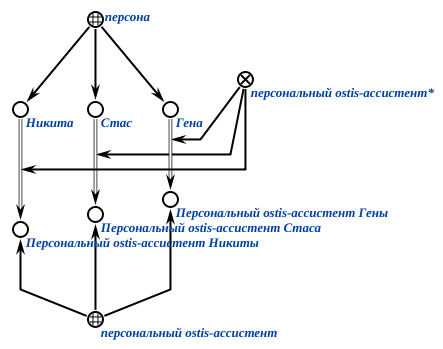
\includegraphics[scale=0.8]{author/part7/chapter_ecosystem/figures/personal_ostis_assistant_example_ru.png}
    \label{fig:ostis_assistant}
\end{figure}

Коллектив, состоящий из персоны и соответствующего ей \textit{персонального ostis-ассистента}, фактически является \textit{минимальным ostis-сообществом}(см. \nameref{fig:ostis_corporate}).

\begin{figure}[H]
    \caption{Пример \textit{минимального ostis-сообщества} в \textit{SCg-коде}}
    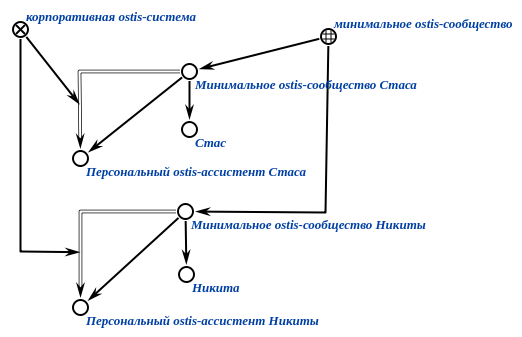
\includegraphics[scale=0.8]{author/part7/chapter_ecosystem/figures/corporate_ostis_system_example_ru.png}
    \label{fig:ostis_corporate}
\end{figure}

Поскольку формально в не \textit{минимальные ostis-сообщества} входят не персоны, а соответствующие им \textit{персональные ostis-ассистенты}, все \textit{ostis-сообщества}, кроме \textit{минимальных ostis-сообществ}, являются \textit{коллективами ostis-систем}.

\textit{корпоративная ostis-система} есть центральная \textit{ostis-система}, осуществляющая координацию, организацию, а также поддержку эволюции деятельности членов соответствующего \textit{ostis-сообщества}. 
\textit{корпоративная ostis-система} является представителем соответствующего \textit{ostis-сообщества} в других \textit{ostis-сообществах}, членом которых оно является(см. \nameref{fig:ostis_community}).

\begin{figure}[H]
    \caption{Пример \textit{корпоративной ostis-системы} \textit{ostis-сообщества} в \textit{SCg-коде}}
    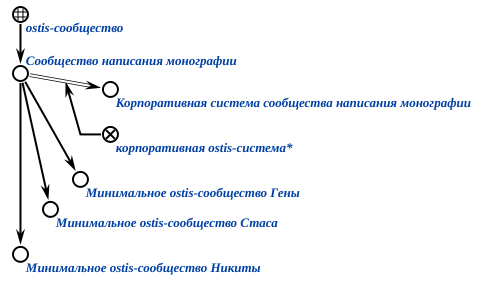
\includegraphics[scale=0.8]{author/part7/chapter_ecosystem/figures/ostis-system collectivity_example_ru.png}
    \label{fig:ostis_community}
\end{figure}

Основным назначением \textit{Корпоративной системы Экосистемы OSTIS} является организация общего взаимодействия при выполнении самых различных видов и областей человеческой деятельности, которые могут быть либо полностью автоматизированными, либо частично автоматизированными, либо вообще неавтоматизированными. 
Из этого следует, что база знаний \textit{Корпоративной системы Экосистемы OSTIS} должна содержать \textit{Общую формальную теорию человеческой деятельности}, включающей в себя типологию видов и областей человеческой деятельности, а также общую методологию этой деятельности.

\begin{SCn}
\scnheader{Деятельность в области Искусственного интеллекта, осуществляемая на основе Технологии OSTIS}
\scnrelfrom{основной продукт}{Экосистема OSTIS}
\begin{scnrelfromlist}{подпроект}
    \scnitem{Проект Метасистемы OSTIS}
    \scnitem{Проект программной реализации абстрактной sc-машины}
    \scnitem{Проект разработки универсального sc-компьютера}
\end{scnrelfromlist}
\end{SCn}

Продуктом человеческой деятельности в области Искусственного интеллекта, осуществляемой на основе \textit{Технологии OSTIS}, является не просто множество \textit{ostis-систем} различного назначения, а Экосистема, состоящая из взаимодействующих \textit{ostis-систем} и их пользователей. 

По назначению \textit{ostis-системы}, входящие в \textit{Экосистему OSTIS}, могут быть:
\begin{textitemize}
    \item ассистентами конкретных пользователей или конкретных пользовательских коллективов;
    \item типовыми встраиваемыми подсистемами \textit{ostis-систем};
    \item системами информационной и инструментальной поддержки проектирования различных компонентов и различных классов \textit{ostis-систем};
    \item системами информационной и инструментальной поддержки проектирования или производства различных классов технических и других искусственно создаваемых систем;
    \item порталами знаний по самым различным научным дисциплинам;
    \item системами автоматизации управления различными сложными объектами (производственными предприятиями, учебными заведениями, кафедрами вузов, конкретными обучаемыми);
    \item интеллектуальными справочными и help-системами;
    \item интеллектуальными робототехническими системами.
\end{textitemize}
Типология \textit{ostis-систем}, являющихся агентом Экосистемы OSTIS, представлена ниже.

\begin{SCn}
\scnheader{ostis-система, являющаяся агентом Экосистемы OSTIS}
\scnsuperset{персональный ostis-ассистент}
\scnsuperset{корпоративная ostis-система}
\scnsuperset{ostis-портал знаний}
\scnsuperset{ostis-система автоматизации проектирования}
\scnsuperset{ostis-система автоматизации производства}
\scnsuperset{ostis-система автоматизации образовательной деятельности}
\begin{scnindent}
	\scnsuperset{обучающаяся ostis-система}
	\scnsuperset{корпоративная ostis-система виртуальной кафедры}
\end{scnindent}
\scnsuperset{ostis-система автоматизации бизнес-деятельности}
\scnsuperset{ostis-система автоматизации управления}
\begin{scnindent}
	\scnsuperset{ostis-система управления проектами соответствующего вида}
	\scnsuperset{ostis-система сенсомоторной координации при выполнении определенного вида сложных действий во внешней среде}
    \begin{scnindent}
        \scnsuperset{ostis-система управления самостоятельным перемещением} 
		\scnsuperset{робота по пересеченной местности}
    \end{scnindent}
\end{scnindent}
\end{SCn}

\begin{SCn}

\bigskip

\begin{scnrelfromlist}{ключевое понятие}
    \scnitem{...}
\end{scnrelfromlist}

\bigskip

\begin{scnrelfromlist}{ключевое знание}
    \scnitem{...}
\end{scnrelfromlist}

\bigskip

\begin{scnrelfromlist}{библиографическая ссылка}
    \scnitem{\scncite{...}}
\end{scnrelfromlist}

\end{SCn}


Без Общей формальной теории интеллектуальных систем невозможно построить набор методов и средств, обеспечивающий комплексную поддержку разработки интеллектуальных компьютерных систем различного назначения и с различным набором навыков, которыми могут обладать интеллектуальные компьютерные системы, но необязательно каждая из них. 
При этом важно не просто построить Общую теорию интеллектуальных систем и довести ее до строгого формального уровня, но также довести представление такой формальной теории до уровня базы знаний соответствующего портала научных знаний.

Целями интеллектуального портала научных знаний являются:
\begin{itemize}
    \item ускорение погружения каждого человека в новые для него научные области при постоянном сохранении общей целостной картины Мира (образовательная цель);
    \item фиксация в систематизированном виде новых научных результатов так, чтобы все основные связи новых результатов с известными были четко обозначены;
    \item автоматизация координации работ по рецензированию новых результатов;
    \item автоматизация анализа текущего состояния базы знаний.
\end{itemize}

Создание интеллектуальных порталов научных знаний, обеспечивающих повышение темпов интеграции и согласования различных точек зрения, – это способ существенного повышения темпов эволюции научно-технической деятельности.
Совместимые порталы научных знаний, реализованные в виде ostis-систем, входящих в Экосистему OSTIS, являются основой новых принципов организации научной деятельности, в которой результатами этой деятельности являются не статьи, монографии, отчеты и другие научно-технические документы, а фрагменты глобальной базы знаний, разработчиками которых являются свободно формируемые научные коллективы, состоящие из специалистов в соответствующих научных дисциплинах. 
С помощью порталов научных знаний осуществляется как координация процесса рецензирования новой научно-технической информации, поступающей от научных работников в базы знаний этих порталов, так и процесс согласования различных точек зрения ученых (в частности, введению и семантической корректировке понятий, а также введению и корректировке терминов, соответствующих различным сущностям).

Реализация семейства семантически совместимых порталов научных знаний в виде совместимых ostis-систем, входящих в состав Экосистемы OSTIS, предполагает разработку иерархической системы семантически согласованных формальных онтологий, соответствующих различным научно-техническим дисциплинам, с четко заданным наследованием свойств описываемых сущностей и с четко заданными междисциплинарными связями, которые описываются связями между соответствующими формальными онтологиями и специфицируемыми ими предметными областями.

Примером портала научных знаний, построенного в виде ostis-системы является Метасистема OSTIS, содержащая все известные на текущий момент знания и навыки, входящие в состав Технологии OSTIS.

\section{Семантически совместимые интеллектуальные корпоративные ostis-системы различного назначения}
{\label{sec_corporate_ostis_system}} 

\begin{SCn}

\bigskip

\begin{scnrelfromlist}{ключевое понятие}
    \scnitem{...}
\end{scnrelfromlist}

\bigskip

\begin{scnrelfromlist}{ключевое знание}
    \scnitem{...}
\end{scnrelfromlist}

\bigskip

\begin{scnrelfromlist}{библиографическая ссылка}
    \scnitem{\scncite{...}}
\end{scnrelfromlist}

\end{SCn}

\textit{Корпоративные системы} представляют собой программные решения, предназначенные для автоматизации бизнес-процессов и управления ресурсами и данными внутри организации. Они могут включать в себя различные подсистемы, такие как управление отношениями с клиентами, управление контентом, управление проектами, управление ресурсами предприятия, управление документами и многое другое.

Роль \textit{корпоративных систем} в современных организациях заключается в обеспечении эффективного управления бизнес-процессами и ресурсами, повышении производительности и качества работы, а также обеспечении прозрачности и оперативности принятия решений на основе актуальных данных.

\textit{Корпоративные системы} могут использоваться для следующих целей:

\begin{textitemize}
    \item автоматизация многих рутинных задач, таких как обработка заказов, управление складом, учет финансовых операций и так далее. Это позволяет сократить время на выполнение задач и уменьшить количество ошибок.
    \item сбор, хранение и обработка данных о бизнес-процессах и ресурсах организации. Это позволяет увеличить точность и оперативность принятия решений, а также обеспечить прозрачность в управлении организацией.
    \item эффективное управление ресурсами организации, такими как финансы, трудовые ресурсы, материальные и технические ресурсы и так далее. Это позволяет сократить затраты на управление ресурсами и повысить эффективность их использования.
    \item управление отношениями с клиентами, автоматизация процессов продаж и обслуживания, а также анализ данных о клиентах. Это позволяет повысить удовлетворенность клиентов и увеличить объемы продаж.
    \item управление проектами, планирование и отслеживание выполнения работ, управление ресурсами и расписание проектов. Это позволяет повысить эффективность выполнения проектов, уменьшить сроки выполнения работ и снизить затраты на проекты.
    \item управление документами, контроль версиями, автоматизация процессов редактирования и утверждения документов. Это позволяет повысить эффективность работы с документами и обеспечить безопасность их хранения и передачи.
\end{textitemize}

Хотя \textit{корпоративные системы} могут принести значительные выгоды для организаций, они также могут столкнуться с рядом проблем, связанных с их внедрением и эксплуатацией. Ниже перечислены некоторые из этих проблем:

\begin{textitemize}
    \item Внедрение корпоративных систем может быть дорогостоящим и трудоемким процессом, который требует значительных ресурсов и экспертизы. Кроме того, многие системы могут потребовать изменения бизнес-процессов и требовать адаптации культуры организации.
    \item Корпоративные системы могут столкнуться с проблемами совместимости с другими системами, используемыми в организации. Это может привести к проблемам с обменом данными и снижению эффективности работы.
    \item Корпоративные системы могут стать мишенью для кибератак, поэтому важно обеспечить безопасность хранения и передачи данных, используемых в системах.
    \item Корпоративные системы могут потребовать значительных затрат на обслуживание и поддержку, включая установку обновлений, устранение ошибок и техническую поддержку.
    \item Внедрение новых корпоративных систем может потребовать обучения персонала, что может быть трудоемким и затратным процессом.
    \item Внедрение корпоративных систем может потребовать изменения бизнес-процессов, что может быть сложным и вызвать сопротивление со стороны сотрудников.
\end{textitemize}

Для создания семантически совместимых интеллектуальных \textit{корпоративных систем} необходимо обеспечить высокую степень гибкости, масштабируемости, автоматизации и интеграции. Это позволит организациям более эффективно управлять ресурсами и данными и повысить их конкурентоспособность на рынке. Для достижения этих целей необходимо использовать современные технологии, такие как аналитика данных, машинное обучение, искусственный интеллект и технологии распределенных вычислений. Кроме того, необходимо учитывать особенности организации и ее бизнес-процессов, чтобы обеспечить максимальную эффективность использования системы. 

Для решения задачи формирования корпоративной системы целесообразно применение \textit{Технологии OSTIS}. \textit{Корпоративная ostis-система} позволяет отслеживать, анализировать и постепенно автоматизировать все процессы обработки данных в рамках ostis-сообщества. 
Такая система действует по следующим принципам:
\begin{textitemize}
    \item интеллектуальные подсистемы (агенты) упорядочивают структуру данных таким образом, что актуальная информация всегда доступна, а устаревшая информация автоматически архивируется или удаляется в соответствии с законами о хранении и защите данных в режиме реального времени;
    \item запросы к системе выполняются в виде простых инструкций, система помогает менеджерам вводить необходимую информацию, осуществляет частичную или полную автоматизацию обновления информации из баз данных, доступных через Интернет;
    \item интеллектуальные подсистемы выполняют структуризацию и классификацию документов и информации для принятия быстрых и правильных решений, автоматически обрабатывает документы и доступные базы данных для отбора ключевой информации, необходимой в данный момент и в будущем;
    \item существующее системное окружение на предприятии может быть легко подключено к системе через открытые интерфейсы, вся информация остается доступной;
    \item все ключевые системы данных синхронизируются с основной системой, данные постоянно сравниваются друг с другом, чтобы избежать потерь;
    \item вся информация доступна в базе знаний, которая является источником данных для рабочих процессов, отчетности и комплексных проверок;
\end{textitemize}

Таким образом, предлагаемая платформа позволяет представить всю ифнормации об \textit{ostis-сообществе} единым целостным образом. 
Достоинствами внедрения предложенной системы являются:
\begin{textitemize}
    \item помощь сбора и оценки информации без преднамеренных искажений или ошибок, связанных с человеческим фактором;
    \item предоставление возможности полного контроля своих данных;
    \item система предоставляет только высококачественные, достоверные и актуальные данные;
    \item цифровое представление всех процессов сообщества обеспечивает интегрированную обработку информации внутри сообщества, что дает полную прозрачность управления, облегчает доступ ко всей информации и ее анализ;
    \item благодаря поддержке интеллектуальных подсистем все необходимые данные из документов, процессов и внешних источников могут быть извлечены, структурированы и грамотно оценены.
\end{textitemize}

\textit{Корпоративные ostis-системы} могут быть применены в различных областях: медицина и здравоохранение, образовательная деятельность широкого профиля, страховой бизнес, промышленная деятельность, административная деятельность, недвижимость, транспорт и так далее.

\section{Персональные ostis-ассистенты пользователей}
{\label{sec_ostis_assistant}} 

\begin{SCn}

\begin{scnrelfromlist}{ключевое понятие}
    \scnitem{персональный ассистент}
    \scnitem{персональный ostis-ассистент}
\end{scnrelfromlist}

\bigskip

\begin{scnrelfromlist}{библиографическая ссылка}
    \scnitem{\scncite{Meurisch2017}}
    \scnitem{\scncite{Meurisch2020}}
    \scnitem{\scncite{Jeni2022}}
    \scnitem{\scncite{Akbar2022}}
\end{scnrelfromlist}

\end{SCn}

Общество должно обеспечивать персональную поддержку каждому человеку, учитывая его индивидуальные особенности, с целью достижения следующих целей:
\begin{textitemize}
    \item максимального уровня физического здоровья, активности и долголетия;
    \item максимального уровня физического комфорта, личного пространства и материального благосостояния;
    \item максимального уровня социального комфорта и защиты прав и свобод.
\end{textitemize}

Для этого должен осуществляться:
\begin{textitemize}
    \item персональный мониторинг каждой личности по всем направлениям;
    \item диагностика и устранение нежелательных отклонений;
    \item оказание своевременной персональной помощи в уточнении направлений дальнейшей эволюции каждой личности.
\end{textitemize}

Необходимо перейти от оказания услуг в решении различных проблем по инициативе самих лиц, столкнувшихся с этими проблемами, к своевременному обнаружению возможности возникновения этих проблем и к соответствующей профилактике. 
Это возможно только при наличии четкой системной организации персонального мониторинга. 

Цифровые \textit{персональные ассистенты} – это программы, основанные на технологиях искусственного интеллекта и машинного обучения, которые помогают пользователям в выполнении повседневных задач, таких как составление расписания, управление контактами, поиск информации, напоминание о важных событиях и так далее (см. \scncite{Meurisch2017}, \scncite{Meurisch2020}, \scncite{Jeni2022}, \scncite{Akbar2022}).

\textit{Персональный ассистент} должен учитывать, что роли пользователя в обществе могут меняться, расширяться, также как и его интересы и цели. 
При этом, все \textit{персональные ассистенты} должны быть семантически совместимыми с целью понимания друг друга, а также обладать способностью самостоятельно взаимодействовать в рамках различных \textit{корпоративных систем}, представляя интересы своих пользователей.

Одной из основных проблем, связанных с реализацией цифровых \textit{персональных ассистентов}, является необходимость точного понимания запросов и задач, поступающих от пользователя. Это может быть вызвано различными факторами, такими как нечеткость и неоднозначность формулировок, использование аббревиатур и сленга, а также многозначность некоторых слов.

Пользователь не обязан знать множество сервисов, из которых он должен выбирать подходящий ему функционал. Комплекс семантически совместимых сервисов должен располагаться "за кадром"{}. Следовательно, все используемые информационные ресурсы и сервисы должны быть семантически совместимы. Выбор подходящего для пользователя ресурса или сервиса должен производить его \textit{персональный ассистент}.

Таким образом, при реализации цифровых \textit{персональных ассистентов} необходимо обеспечить их масштабируемость и адаптивность к потребностям пользователей. Это означает, что система должна быть способна автоматически адаптироваться к изменениям в поведении пользователя, учитывая его предпочтения, особенности работы и другие факторы.

\textit{Технология OSTIS} позволяет создавать семантически совместимые системы, которые способны обрабатывать запросы и задачи пользователей, учитывая их контекст и смысл. Это достигается за счет использования семантических сетей, которые позволяют описывать знания и связи между ними. Кроме того, \textit{технология OSTIS} обеспечивает масштабируемость и гибкость системы, что позволяет ей адаптироваться к изменениям в поведении пользователей и изменениям в их потребностях.

\textit{Персональный ostis-ассистент} есть \textit{ostis-система}, являющаяся \textit{персональным ассистентом} пользователя в рамках \textit{Экосистемы OSTIS}.
Такая система предоставляет возможности:
\begin{textitemize}
    \item анализа деятельности пользователя и формирования рекомендаций по ее оптимизации;
    \item адаптации под настроение пользователя, его личностные качества, общую окружающую обстановку, задачи, которые чаще всего решает пользователь;
    \item перманентного обучения самого ассистента в процессе решения новых задач, при этом обучаемость потенциально не ограничена;
    \item вести диалог с пользователем на естественном языке, в том числе в речевой форме;
    \item отвечать на вопросы различных классов, при этом если системе что-то не понятно, то она сама может задавать встречные вопросы;
    \item автономного получения информации от всей окружающей среды, а не только от пользователя (в текстовой или речевой форме).
\end{textitemize}

При этом система может как анализировать доступные информационные источники (например, в интернете), так и анализировать окружающий ее физический мир, например, окружающие предметы или внешний вид пользователя.

Достоинства \textit{персонального ostis-ассистента}:
\begin{textitemize}
    \item пользователю нет необходимости хранить разную информацию в разной форме в разных местах, вся информация хранится в единой базе знаний компактно и без дублирований;
    \item благодаря неограниченной обучаемости ассистенты могут потенциально автоматизировать практически любую деятельность, а не только самую рутинную;
    \item благодаря базе знаний, ее структуризации и средствам поиска информации в базе знаний пользователь может получить более точную информацию более быстро.
\end{textitemize}

\textit{Персональные ассистенты} имеют самое различное назначение и могут быть использованы для самых различных категорий пользователей (пациент, юридическое обслуживание, административное обслуживание, покупатель, потребитель различных услуг). \textit{Персональный ostis-ассистент} может использовать знания и данные, хранящиеся в других \textit{ostis-системах}, таких как \textit{корпоративные ostis-системы}, чтобы предоставлять пользователю более полную и актуальную информацию. Это может быть особенно полезно для пользователей, которые работают с большим количеством данных и информации. \textit{Персональный ostis-ассистент} автоматически интегрируется с другими \textit{ostis-системами}, что позволяет ему более эффективно работать с данными и информацией. Он может использовать технологии машинного обучения и искусственного интеллекта для адаптации к поведению пользователя и улучшения его производительности и эффективности. \textit{Персональный ostis-ассистент} может быть создан и настроен с учетом конкретных потребностей организации и ее процессов, что может привести к значительным экономическим и производственным преимуществам.

Таким образом, \textit{персональные ostis-ассистенты} обладают рядом преимуществ по сравнению с другими реализациями цифровых \textit{персональных ассистентов}, таких как более точное понимание запросов и задач пользователей, доступ к актуальным данным и информации, автоматическая интеграция с другими \textit{ostis-системами} в рамках \textit{Экосистемы OSTIS} и адаптация к потребностям организации и ее процессов.


%%%%%%%%%%%%%%%%%%%%%%%%% referenc.tex %%%%%%%%%%%%%%%%%%%%%%%%%%%%%%
% sample references
% %
% Use this file as a template for your own input.
%
%%%%%%%%%%%%%%%%%%%%%%%% Springer-Verlag %%%%%%%%%%%%%%%%%%%%%%%%%%
%
% BibTeX users please use
% \bibliographystyle{}
% \bibliography{}
%
\biblstarthook{In view of the parallel print and (chapter-wise) online publication of your book at \url{www.springerlink.com} it has been decided that -- as a genreral rule --  references should be sorted chapter-wise and placed at the end of the individual chapters. However, upon agreement with your contact at Springer you may list your references in a single seperate chapter at the end of your book. Deactivate the class option \texttt{sectrefs} and the \texttt{thebibliography} environment will be put out as a chapter of its own.\\\indent
References may be \textit{cited} in the text either by number (preferred) or by author/year.\footnote{Make sure that all references from the list are cited in the text. Those not cited should be moved to a separate \textit{Further Reading} section or chapter.} If the citatiion in the text is numbered, the reference list should be arranged in ascending order. If the citation in the text is author/year, the reference list should be \textit{sorted} alphabetically and if there are several works by the same author, the following order should be used:
\begin{enumerate}
\item all works by the author alone, ordered chronologically by year of publication
\item all works by the author with a coauthor, ordered alphabetically by coauthor
\item all works by the author with several coauthors, ordered chronologically by year of publication.
\end{enumerate}
The \textit{styling} of references\footnote{Always use the standard abbreviation of a journal's name according to the ISSN \textit{List of Title Word Abbreviations}, see \url{http://www.issn.org/en/node/344}} depends on the subject of your book:
\begin{itemize}
\item The \textit{two} recommended styles for references in books on \textit{mathematical, physical, statistical and computer sciences} are depicted in ~\cite{science-contrib, science-online, science-mono, science-journal, science-DOI} and ~\cite{phys-online, phys-mono, phys-journal, phys-DOI, phys-contrib}.
\item Examples of the most commonly used reference style in books on \textit{Psychology, Social Sciences} are~\cite{psysoc-mono, psysoc-online,psysoc-journal, psysoc-contrib, psysoc-DOI}.
\item Examples for references in books on \textit{Humanities, Linguistics, Philosophy} are~\cite{humlinphil-journal, humlinphil-contrib, humlinphil-mono, humlinphil-online, humlinphil-DOI}.
\item Examples of the basic Springer style used in publications on a wide range of subjects such as \textit{Computer Science, Economics, Engineering, Geosciences, Life Sciences, Medicine, Biomedicine} are ~\cite{basic-contrib, basic-online, basic-journal, basic-DOI, basic-mono}. 
\end{itemize}
}

\begin{thebibliography}{99.}%
% and use \bibitem to create references.
%
% Use the following syntax and markup for your references if 
% the subject of your book is from the field 
% "Mathematics, Physics, Statistics, Computer Science"
%
% Contribution 
\bibitem{science-contrib} Broy, M.: Software engineering --- from auxiliary to key technologies. In: Broy, M., Dener, E. (eds.) Software Pioneers, pp. 10-13. Springer, Heidelberg (2002)
%
% Online Document
\bibitem{science-online} Dod, J.: Effective substances. In: The Dictionary of Substances and Their Effects. Royal Society of Chemistry (1999) Available via DIALOG. \\
\url{http://www.rsc.org/dose/title of subordinate document. Cited 15 Jan 1999}
%
% Monograph
\bibitem{science-mono} Geddes, K.O., Czapor, S.R., Labahn, G.: Algorithms for Computer Algebra. Kluwer, Boston (1992) 
%
% Journal article
\bibitem{science-journal} Hamburger, C.: Quasimonotonicity, regularity and duality for nonlinear systems of partial differential equations. Ann. Mat. Pura. Appl. \textbf{169}, 321--354 (1995)
%
% Journal article by DOI
\bibitem{science-DOI} Slifka, M.K., Whitton, J.L.: Clinical implications of dysregulated cytokine production. J. Mol. Med. (2000) doi: 10.1007/s001090000086 
%
\bigskip

% Use the following (APS) syntax and markup for your references if 
% the subject of your book is from the field 
% "Mathematics, Physics, Statistics, Computer Science"
%
% Online Document
\bibitem{phys-online} J. Dod, in \textit{The Dictionary of Substances and Their Effects}, Royal Society of Chemistry. (Available via DIALOG, 1999), 
\url{http://www.rsc.org/dose/title of subordinate document. Cited 15 Jan 1999}
%
% Monograph
\bibitem{phys-mono} H. Ibach, H. L\"uth, \textit{Solid-State Physics}, 2nd edn. (Springer, New York, 1996), pp. 45-56 
%
% Journal article
\bibitem{phys-journal} S. Preuss, A. Demchuk Jr., M. Stuke, Appl. Phys. A \textbf{61}
%
% Journal article by DOI
\bibitem{phys-DOI} M.K. Slifka, J.L. Whitton, J. Mol. Med., doi: 10.1007/s001090000086
%
% Contribution 
\bibitem{phys-contrib} S.E. Smith, in \textit{Neuromuscular Junction}, ed. by E. Zaimis. Handbook of Experimental Pharmacology, vol 42 (Springer, Heidelberg, 1976), p. 593
%
\bigskip
%
% Use the following syntax and markup for your references if 
% the subject of your book is from the field 
% "Psychology, Social Sciences"
%
%
% Monograph
\bibitem{psysoc-mono} Calfee, R.~C., \& Valencia, R.~R. (1991). \textit{APA guide to preparing manuscripts for journal publication.} Washington, DC: American Psychological Association.
%
% Online Document
\bibitem{psysoc-online} Dod, J. (1999). Effective substances. In: The dictionary of substances and their effects. Royal Society of Chemistry. Available via DIALOG. \\
\url{http://www.rsc.org/dose/Effective substances.} Cited 15 Jan 1999.
%
% Journal article
\bibitem{psysoc-journal} Harris, M., Karper, E., Stacks, G., Hoffman, D., DeNiro, R., Cruz, P., et al. (2001). Writing labs and the Hollywood connection. \textit{J Film} Writing, 44(3), 213--245.
%
% Contribution 
\bibitem{psysoc-contrib} O'Neil, J.~M., \& Egan, J. (1992). Men's and women's gender role journeys: Metaphor for healing, transition, and transformation. In B.~R. Wainrig (Ed.), \textit{Gender issues across the life cycle} (pp. 107--123). New York: Springer.
%
% Journal article by DOI
\bibitem{psysoc-DOI}Kreger, M., Brindis, C.D., Manuel, D.M., Sassoubre, L. (2007). Lessons learned in systems change initiatives: benchmarks and indicators. \textit{American Journal of Community Psychology}, doi: 10.1007/s10464-007-9108-14.
%
%
% Use the following syntax and markup for your references if 
% the subject of your book is from the field 
% "Humanities, Linguistics, Philosophy"
%
\bigskip
%
% Journal article
\bibitem{humlinphil-journal} Alber John, Daniel C. O'Connell, and Sabine Kowal. 2002. Personal perspective in TV interviews. \textit{Pragmatics} 12:257--271
%
% Contribution 
\bibitem{humlinphil-contrib} Cameron, Deborah. 1997. Theoretical debates in feminist linguistics: Questions of sex and gender. In \textit{Gender and discourse}, ed. Ruth Wodak, 99--119. London: Sage Publications.
%
% Monograph
\bibitem{humlinphil-mono} Cameron, Deborah. 1985. \textit{Feminism and linguistic theory.} New York: St. Martin's Press.
%
% Online Document
\bibitem{humlinphil-online} Dod, Jake. 1999. Effective substances. In: The dictionary of substances and their effects. Royal Society of Chemistry. Available via DIALOG. \\
http://www.rsc.org/dose/title of subordinate document. Cited 15 Jan 1999
%
% Journal article by DOI
\bibitem{humlinphil-DOI} Suleiman, Camelia, Daniel C. O'Connell, and Sabine Kowal. 2002. `If you and I, if we, in this later day, lose that sacred fire...': Perspective in political interviews. \textit{Journal of Psycholinguistic Research}. doi: 10.1023/A:1015592129296.
%
%
%
\bigskip
%
%
% Use the following syntax and markup for your references if 
% the subject of your book is from the field 
% "Computer Science, Economics, Engineering, Geosciences, Life Sciences"
%
%
% Contribution 
\bibitem{basic-contrib} Brown B, Aaron M (2001) The politics of nature. In: Smith J (ed) The rise of modern genomics, 3rd edn. Wiley, New York 
%
% Online Document
\bibitem{basic-online} Dod J (1999) Effective Substances. In: The dictionary of substances and their effects. Royal Society of Chemistry. Available via DIALOG. \\
\url{http://www.rsc.org/dose/title of subordinate document. Cited 15 Jan 1999}
%
% Journal article by DOI
\bibitem{basic-DOI} Slifka MK, Whitton JL (2000) Clinical implications of dysregulated cytokine production. J Mol Med, doi: 10.1007/s001090000086
%
% Journal article
\bibitem{basic-journal} Smith J, Jones M Jr, Houghton L et al (1999) Future of health insurance. N Engl J Med 965:325--329
%
% Monograph
\bibitem{basic-mono} South J, Blass B (2001) The future of modern genomics. Blackwell, London 
%
\end{thebibliography}


\section*{Заключение к Главе \ref{chapter_ecosystem}}

\textit{Экосистема OSTIS} представляет собой саморазвивающуюся сеть \textit{ostis-систем}, которая обеспечивает комплексную автоматизацию всевозможных видов и областей человеческой деятельности. 

\textit{Экосистема OSTIS} является следующим этапом развития человеческого общества, обеспечивающий существенное повышение уровня общественного, коллективного интеллекта путем преобразования человеческого общества в экосистему, состоящую из людей и семантически совместимых интеллектуальных систем. 
\textit{Экосистема OSTIS} --- предлагаемый подход к реализации \textit{smart-общества} или Общества 5.0, построенного на основе \textit{Технологии OSTIS}.

Сверхзадачей \textit{Экосистемы OSTIS} является не просто комплексная автоматизация всех видов человеческой деятельности (только тех видов деятельности, автоматизация которых целесообразна), но и существенное повышение уровня интеллекта различных человеко-машинных сообществ и всего человеческого общества в целом.
